\subsection{Oberflächenentwurf}
\label{sec:Oberflaechenentwuf}

Ein Oberflächenentwurf, auch Mockup genannt, eignet sich besonders in
IT-Projekten für einen ersten Grobentwurf der Benutzeroberfläche des zu
entwickelnden Systems. Ein solcher Oberflächenentwurf beinhaltet die wichtigsten
Benutzerelemente, mit denen die Funktionen des Systems erfüllt werden können.
Das Design und das Layout der Benutzerelemente ist dabei zweitrangig. Ein
Oberflächenentwurf dient in erster Linie dazu, das System für die Entwickler zu
visualisieren. Dies ist besonders von Vorteil, wenn mehrere Personen an der
Entwicklung beteiligt sind. In diesem Fall vermittelt der Oberflächenentwurf ein
einheitliches Bild des zu realisierenden Systems an alle beteiligten
Entwickler. Dieser erste Eindruck vom Endprodukt ist auch für die Auftraggeber
eines Projektes von großem Interesse. Der Oberflächenentwurf dient somit im
zweiten Schritt auch dem Auftraggeber und der Kommunikation zwischen
Auftraggeber und Entwicklerteam. Funktionsvorstellungen und Erweiterung können
mit Hilfe eines Oberflächenentwurfs direkt an einem Modell festgemacht werden.
Auf diese Weise können Fehlentwicklungen von Beginn des Projektes an verhindert
werden.

\subsubsection{Benutzeransicht}
\label{sec:Benutzeransicht}

Ein erster Oberflächenentwurf der Benutzeransicht des vorliegenden Projektes ist in folgender Abbildung zu sehen.

\begin{figure}[htb]
\centering
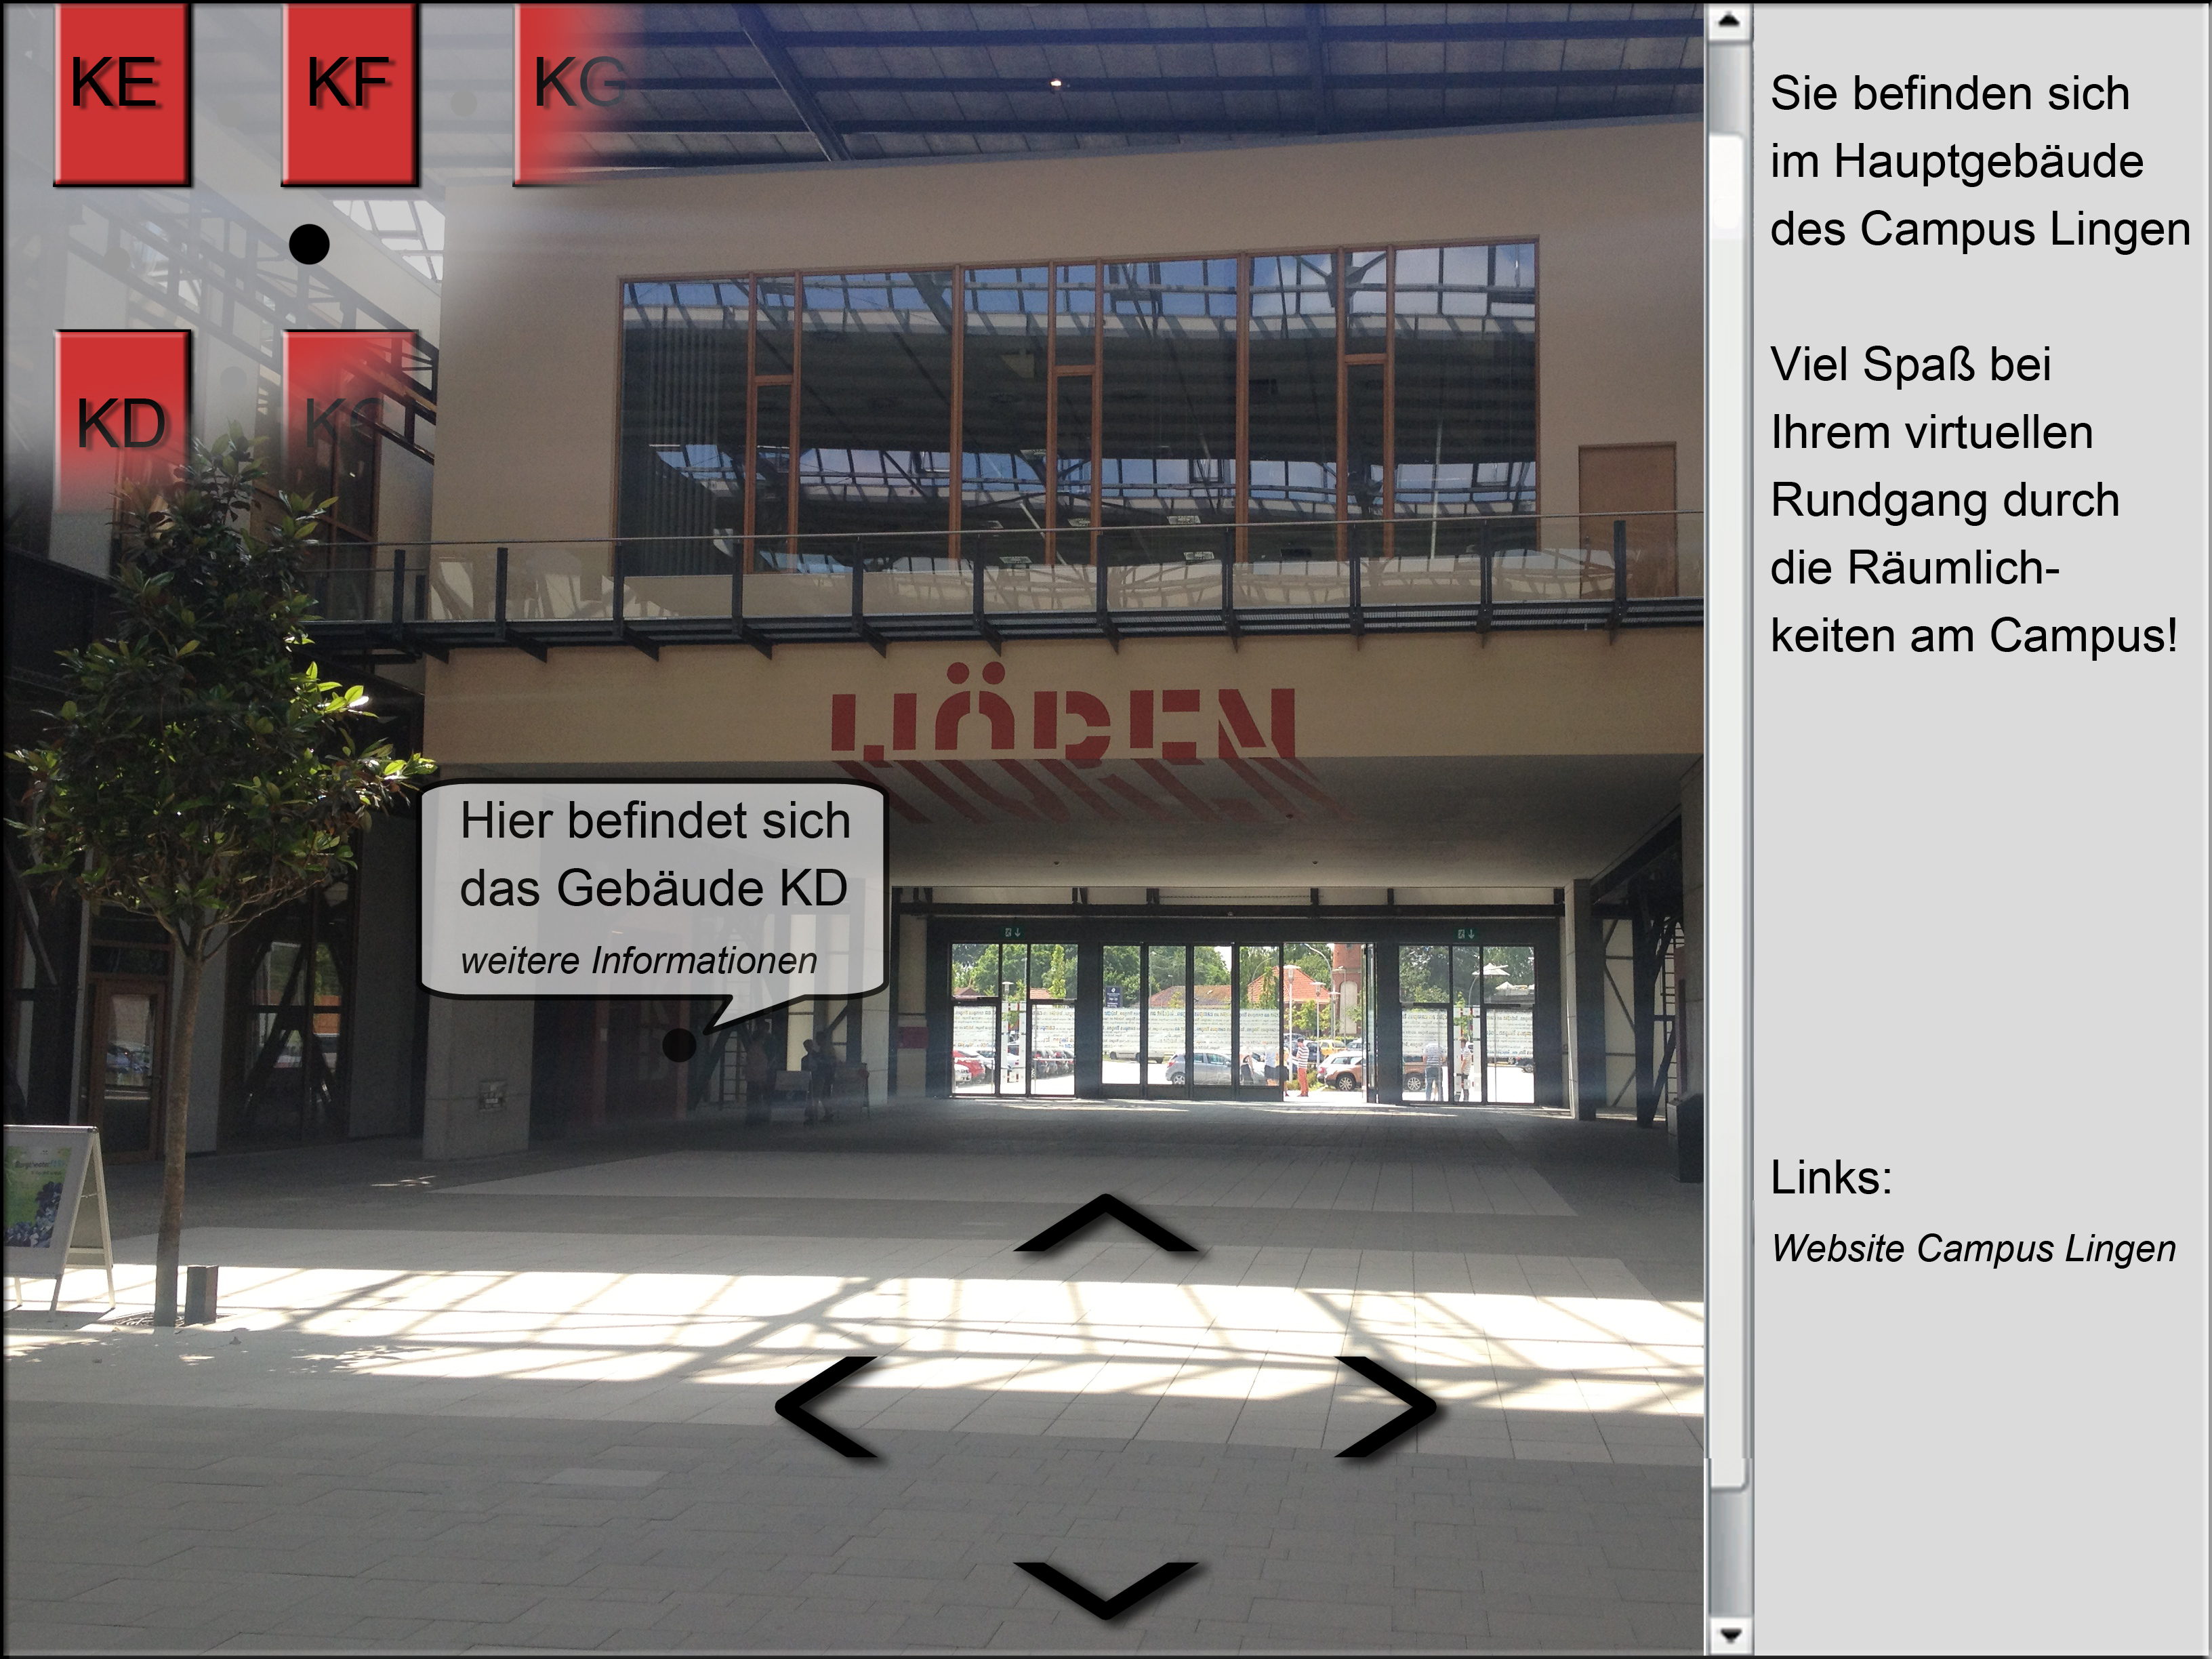
\includegraphics[width=1.0\textwidth]{MockupFrontend.jpg}
\caption[Mockup Benutzeransicht]{Oberflächenentwurf der
Benutzeransicht\protect\footnotemark}
\label{fig:MockupFrontend}
\end{figure}
\footnotetext{Quelle: Eigene Darstellung}

In diesem Mockup sind vier Elemente dargestellt, deren Funktion im Folgenden erläutert wird.

\begin{itemize}
 \item Ein 360-Grad Panorama
 \item Ein Steuerkreuz
 \item Eine kleine Übersichtskarte (Minimap)
 \item Ein Informationsfenster
\end{itemize}

Das \textbf{360-Grad Panorama} ist zentrales Element des Projektes. Dieses Panorama stellt einen Blickwinkel dar, von dem aus sich ein Benutzer den Campus Lingen ansehen kann. Von diesem Blickwinkel aus kann sich der Benutzer virtuell um die Vertikalachse der Fotoaufnahme drehen und dabei alles in diesem Blickwinkel betrachten. Er kann zudem die Aufnahme um 180-Grad horizontal drehen. Ein Benutzer hat damit von einen Standpunkt aus einen vollen Rundumblick.

Mit dem \textbf{Steuerkreuz} am unteren Rand des Panoramas kann ein Benutzer zu einem anderen Aufnahmepunkt wechseln. Er erhält damit einen Einblick aus einem anderen Blickwinkel und kann sich in diesem wiederum frei umsehen. Die Pfeile des Steuerkreuzes zeigen dabei zu jeder Panoramaaufnahme, die von der aktuellen Position erreichbar ist.

Die \textbf{Minimap} ist in einer der Ecken des Panoramas platziert und erfüllt zwei Aufgaben. Zum einen dient sie der Übersichtlichkeit und Orientierung des Benutzers. Sie zeigt an welcher Aufnahmeposition sich der Benutzer aktuell am Campus befindet (im Oberflächentwurf durch einen schwarzen Punkt gekennzeichnet). Hierdurch wird neben dem Einblick in die Räumlichkeiten des Campus auch ein Bild des Aufbaus vermittelt.
Zum anderen kann die Minimap, genau wie die Pfeile des Steuerkreuzes, zum Navigieren zu anderen Aufnahmen genutzt werden. Dazu werden alle Aufnahmepositionen, die sich im Sichtfeld des dargestellten Ausschnittes befinden, farblich hervorgehoben. Durch anklicken einer solchen Markierung wird der Benutzer in eine andere Aufnahmeposition versetzt. Beim wechseln der Aufnahmeposition verändert sich dabei auch der dargestellte Ausschnitt der Minimap.

Das \textbf{Informationsfenster} zeigt zu guter Letzt interessante Informationen zum aktuellen Panorama an. Im obigen Oberflächenentwurf sind zwei solcher Informationsfenster dargestellt (am rechten Rand und oberhalb des Steuerkreuzes). Diese Darstellungsformen sind als alternativ zu betrachten. Die Art der Informationsdarstellung ist zum Zeitpunkt des Öberflächenentwurfs noch nicht eindeutig festgelegt. Inhalt dieser Informationsfenster können dabei Interessante Projekte einzelner Studiengänge, Öffnungszeiten von Räumlichkeiten oder Wissenwertes aus dem Studienalltag sein. Die Anzeige der Informationsfenster ist dabei in einer Art Popup gedacht. Das heißt sie sollen nicht permanent angezeigt werden, sondern erscheinen erst durch Klick des Benutzers auf einen Button. Dadurch wird das Panorama und damit der Blick des Benutzers nicht durch störende Anzeigen eingeschränkt.
\subsubsection{Administrationsbereich}
\label{sec:UmsetzungAdministrationsbereich}

Der entwickelte Prototyp stellt eine erste lauffähige Version einer Benutzeransicht dar. Der nächste Entwicklungsschritt ist die Implementierung des Administrationsbereiche und die Bereitstellung von APIs. Aufbauend auf gepflegten Ìnformationen im Administrationsbereich wird der Prototyp dann um dynamische Funktionalität erweitert. Das heißt die angezeigten Panoramas und die benachbarten Panoramas werden über eine API angefragt, die die Informationen aus der Datenbank lädt. Der Implementierungsprozess des Administrationsbereiches wird dabei sukzessiv anhand der vorgestellten Anwendungsfällen (siehe \nameref{sec:Adminstratoranwendungen} auf Seite \pageref{sec:Adminstratoranwendungen}) realisiert. Prioresiert werden dabei die Anwendungsfälle, die die Verwaltung der Panoramas, Infotexte und die Übersichtskarte betreffen (AFA05 bis AFA17).

Bevor mit der Implementierung begonnen werden kann wird noch ein einheitliches Design festgelegt, dass vor allem dem späteren Administrator das Verständnis erleichtert. Zu diesem einheitlichen Design Konzept zählt zum Beispiel das Farbschema von Buttons. So wurde beispielsweise festgelegt, dass ein roter Button immer das Löschen eines Datensatzes signalisiert und ein grüner immer das speichern eines Datensatzes. Darüber hinaus wurde entschieden die Gestaltung von Buttons, Informationsfenster und ähnlichem mit dem CSS\footnotemark\ Framework Bootstrap\footnotemark\ zu realisieren. Dadurch ist gewährleistet, dass alle Steuerungselemente in allen Browsern gleich aussehen und der Administrator Elemente durch ihr Aussehen wiedererkennen und darüber auf ihre Benutzung schließen kann. Durch diese Entscheidungen wird die Usability der Software erhöht und der Aufwand der zu erstellenden Dokumentation verringert.

\footnotetext{CSS steht für Cascading Style Sheets und beschreibt eine Skriptsprache, die dazu dient HTML-Elemente in Form und Farbe zu verändern.}

\footnotetext{Bootstrap ist ein open Source Projekt, in dem einheitlich das Design von verschiedenen HTML-Elemente definiert ist. Bootstrap ist ein Projekt des Internetkonzerns Twitter und ist besonders dafür geeignet ein einheitliches Look and Feel einer Webseite in allen Browsern zu erzeugen.}

Aufbauend auf Administratoranwendungsfällen und Designkonzept werden Tickets erstellt, deren Inhalt die Implementierung der Infotext- und Fotoverwaltung ist. Zur Verdeutlichung der eingesetzten Technologien und des Entwicklunsablaufs wird im Folgenden eine stark vereinfachte Fotoverwaltungsseite implementiert. Implementiert werden soll eine Seite, die alle Fotos der Datenbank mit Namen und Beschreibung anzeigt. Zustätzlich soll es dem Administrator möglich sein auf den Namen eines Fotos zu klicken, woraufhin ihm weitere Informationen angezeigt werden.

Zur Implementierung dieses Szenarios wird zunächst ein HTML-Dokument angefertigt, dass das Grundgerüst der Fotoverwaltung darstellt. In diesem Grundgerüst könnten bestimmte Elemente, wie zum Beispiel die Navigationsbar am oberen Rand (vergleiche \abbildung{MockupBackend}) der Seite oder der Titel der Seite, statisch codiert werden. Zur Vereinfachung soll aber nur der Titel der Seite gesetzt werden und eine Überschrift. Das folgende \listing{HTML_Anwendungsbeispiel} zeigt das angefertigte HTML-Dokument.

\lstinputlisting[language=HTML,caption={statisches HTML},label={lst:HTML_Anwendungsbeispiel}]{Listings/HTML_Anwendungsbeispiel.html}

Im Anschluss daran muss die Seite um dynamisch generierten Inhalt erweitert werden. Dynamischer Inhalt ist im gegeben Anwendungsfall das Anzeigen aller Fotos, die bereits in der Datenbank sind. Um dieses Verhalten zu realisieren muss eine Anfrage an die Datenbank gestellt werden und danach muss für jeden Eintrag in der Datenbank HTML Quellcode geschrieben werden. Das nachfolgende \listing{HTML mit PHP} zeigt die Implementierung mit PHP.

\lstinputlisting[language=HTML,caption={Dynamisches schreiben von HTML mit PHP},label={lst:HTML mit PHP}]{Listings/HTML_mit_PHP.php}

Zu sehen ist die Anfrage an die Datenbank, die durch die PHP-Funktion "`mysql\_query"' (Zeile 5) realisiert wird, das Durchlaufen jeden Datenbanksatzes in einer Schleife (Zeile 6ff.) und das schreiben von HTML mit dem PHP "`echo"'-Befehl.

Zum Abschluss wird das klicken auf den Fotonamen implementiert. Diese Benutzerinteraktion kann am besten auf dem Clientsystem des Benutzers (Internetbrowser) mit Javascript verarbeitet werden, da keine weiteren Informationen vom Server benötigt werden und zusätzliche Anfragen so vermieden werden. Javascript-Routinen werden meistens als Funktionen formuliert, die aufgerufen werden, wenn ein bestimmtes Ereignis eintritt. Im \listing{HTML mit PHP} ist ein solcher Funktionsaufruf in Zeile 9 zu sehen. Die Funktion "`toggleDescription"' wird aufgerufen sobald auf das <p>-Tag geklickt wird. Als Parameter wird dieser Funktion das eigene HTML-Element, also das <p>-Tag, mitgegeben. Die Javascript-Funktion ist in \listing{Javascript Snippet} dargestellt.

\lstinputlisting[language=JavaScript,caption={Auf Benutzerinteraktion reagieren mit Javascript},label={lst:Javascript Snippet}]{Listings/Javascript_Snippet.js}

Alle dargestellten Listings könnten dabei in einem Dokument stehen, das vom dem Administrator über seinen Internetbrowser angefragt wird.
Wie bereits erwähnt ist diese Darstellung der Implementierung sehr stark vereinfacht. Die Quelldateien, die die Fotoverwaltung im vorliegenden Projekt implementieren, sind zu umfangreich, um sie an dieser Stelle zu präsentieren. Die implementierte Fotoverwaltung wird in folgendem Bildschirmfoto zur Veranschaulichung dargestellt:

%TODO: Bildschirmfoto ohne Pixelfehler machen.
\begin{figure}[htb]
\centering
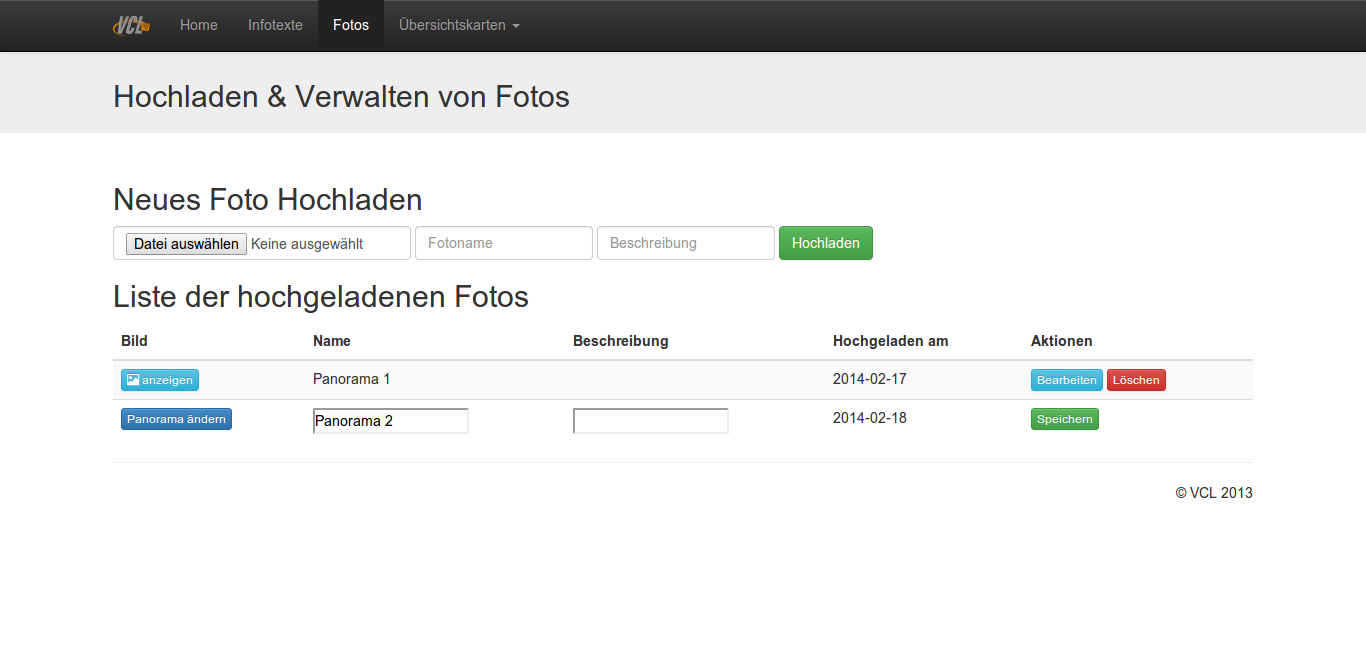
\includegraphics[width=1.0\textwidth]{Fotoverwaltung.png}
\caption[Fotoverwaltung]{Bildschirmfoto der implementierten Fotoverwaltung}
\label{fig:Fotoverwaltung}
\end{figure}

In einem solchen Entwicklungszyklus wurde auch die Verwaltung der Infotexte und die Übersichtskarte implementiert. Bildschirmfotos dieser Bereiche sind im Anhang dargstellt, siehe \abbildung{ScreenshotInfotext}, \abbildung{ScreenshotUebersichtskarte}.